%\documentclass{article}
\documentclass[31pt]{article}
\usepackage[utf8]{inputenc}

\title{MSD+GC sync}
\author{Álvaro Díez González-Pardo }
\date{August 2016}

\usepackage{natbib}
\usepackage{graphicx}
\DeclareGraphicsExtensions{.pdf,.png,.jpg} % Graphics type


\begin{document}

\maketitle

\section{Prerequisites}

GC and MSD should be able to comunicate 

\newpage

\section{Preparing MSD to be started manually}
First we need to put the MSD in PreRun state so that it's ready to start a measurement and it's waiting for the start signal to be received. To do this in a safe manner one should edit the method by clicking \texttt{Method -> Edit Entire Method...}s shown in the picture.

\begin{figure}[h!]
\centering
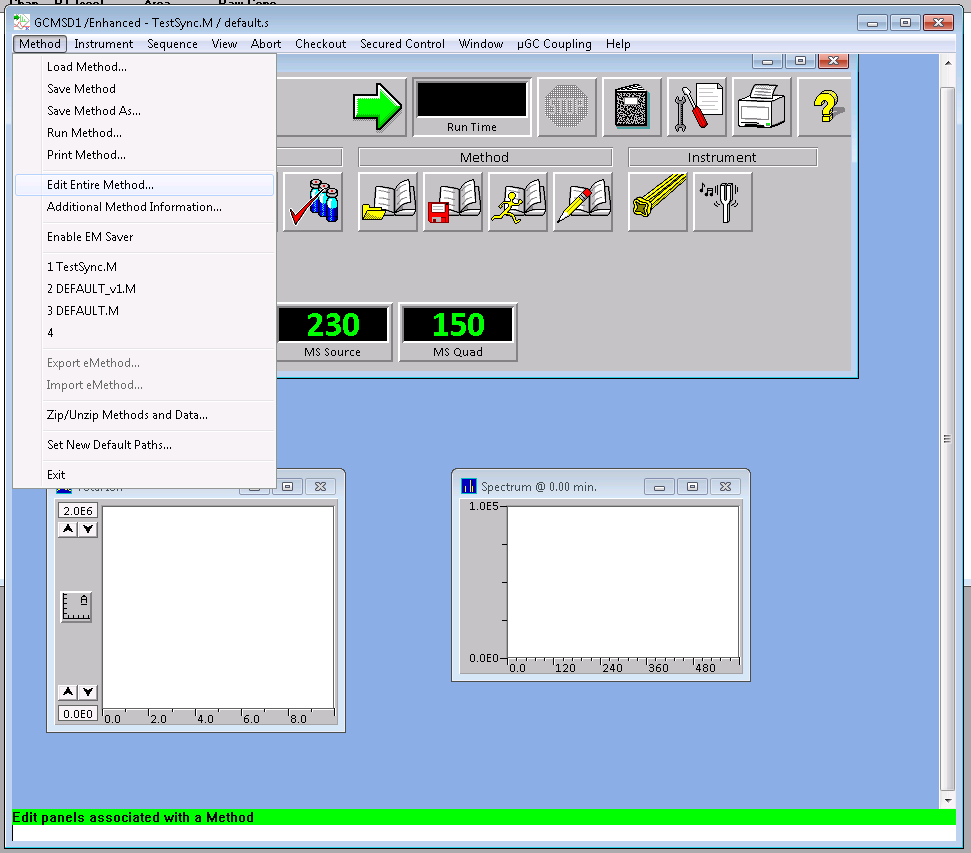
\includegraphics[width=1.3\textwidth]{1-EditMethod.png}
\label{fig:univerise}
\end{figure}

\newpage

A new window will appear and we select only \texttt{Instrument/Adquisition} option and hit \texttt{OK} as shown in the following screen capture:

\begin{figure}[h]
\centering
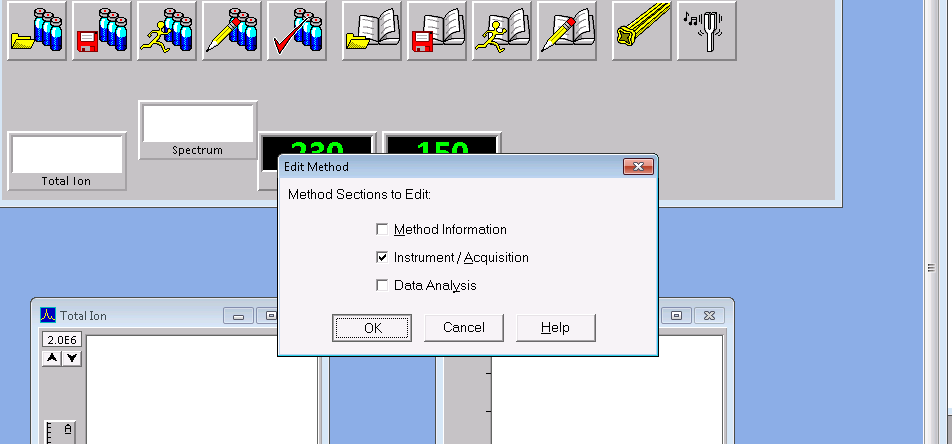
\includegraphics[width=1.1\textwidth]{2Instrument_adq.png}
\label{fig:univerise}
\end{figure}

Another window should appear in the screen. Under \texttt{Injection Source} options we select \texttt{Manual} and hit \texttt{OK} again

\begin{figure}[h]
\centering
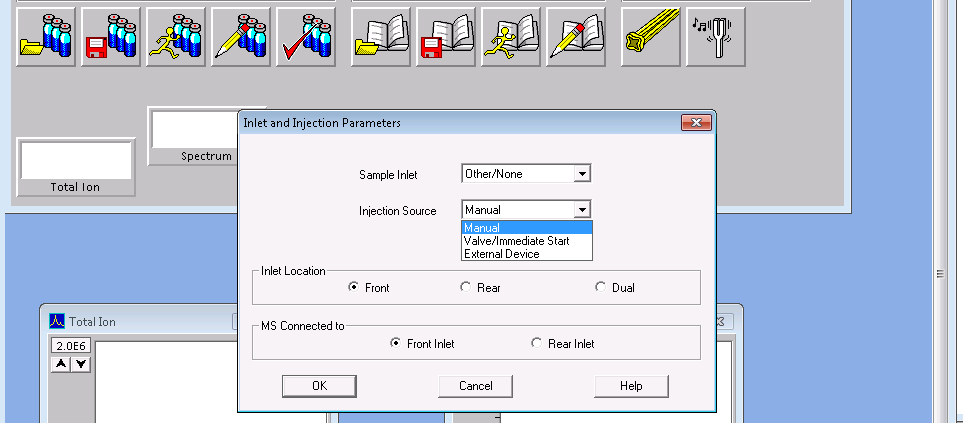
\includegraphics[width=1.1\textwidth]{3ManualStart.png}
\label{fig:univerise}
\end{figure}

From this point on one should click \texttt{OK} or \texttt{Next} or similar buttons until the process of editing the method is completed. Now the MSD is almost ready to be set in PreRun.

\newpage

Open Soprane without closing the Chemstation software and start an analysis that will trigger also the MSD. For that you should check that Coupling is enabled in the options and that the text MSD is displayed on the lower part of the Soprane window. For better understanding a picture of both checks is presented below these lines.

\begin{figure}[h]
\centering
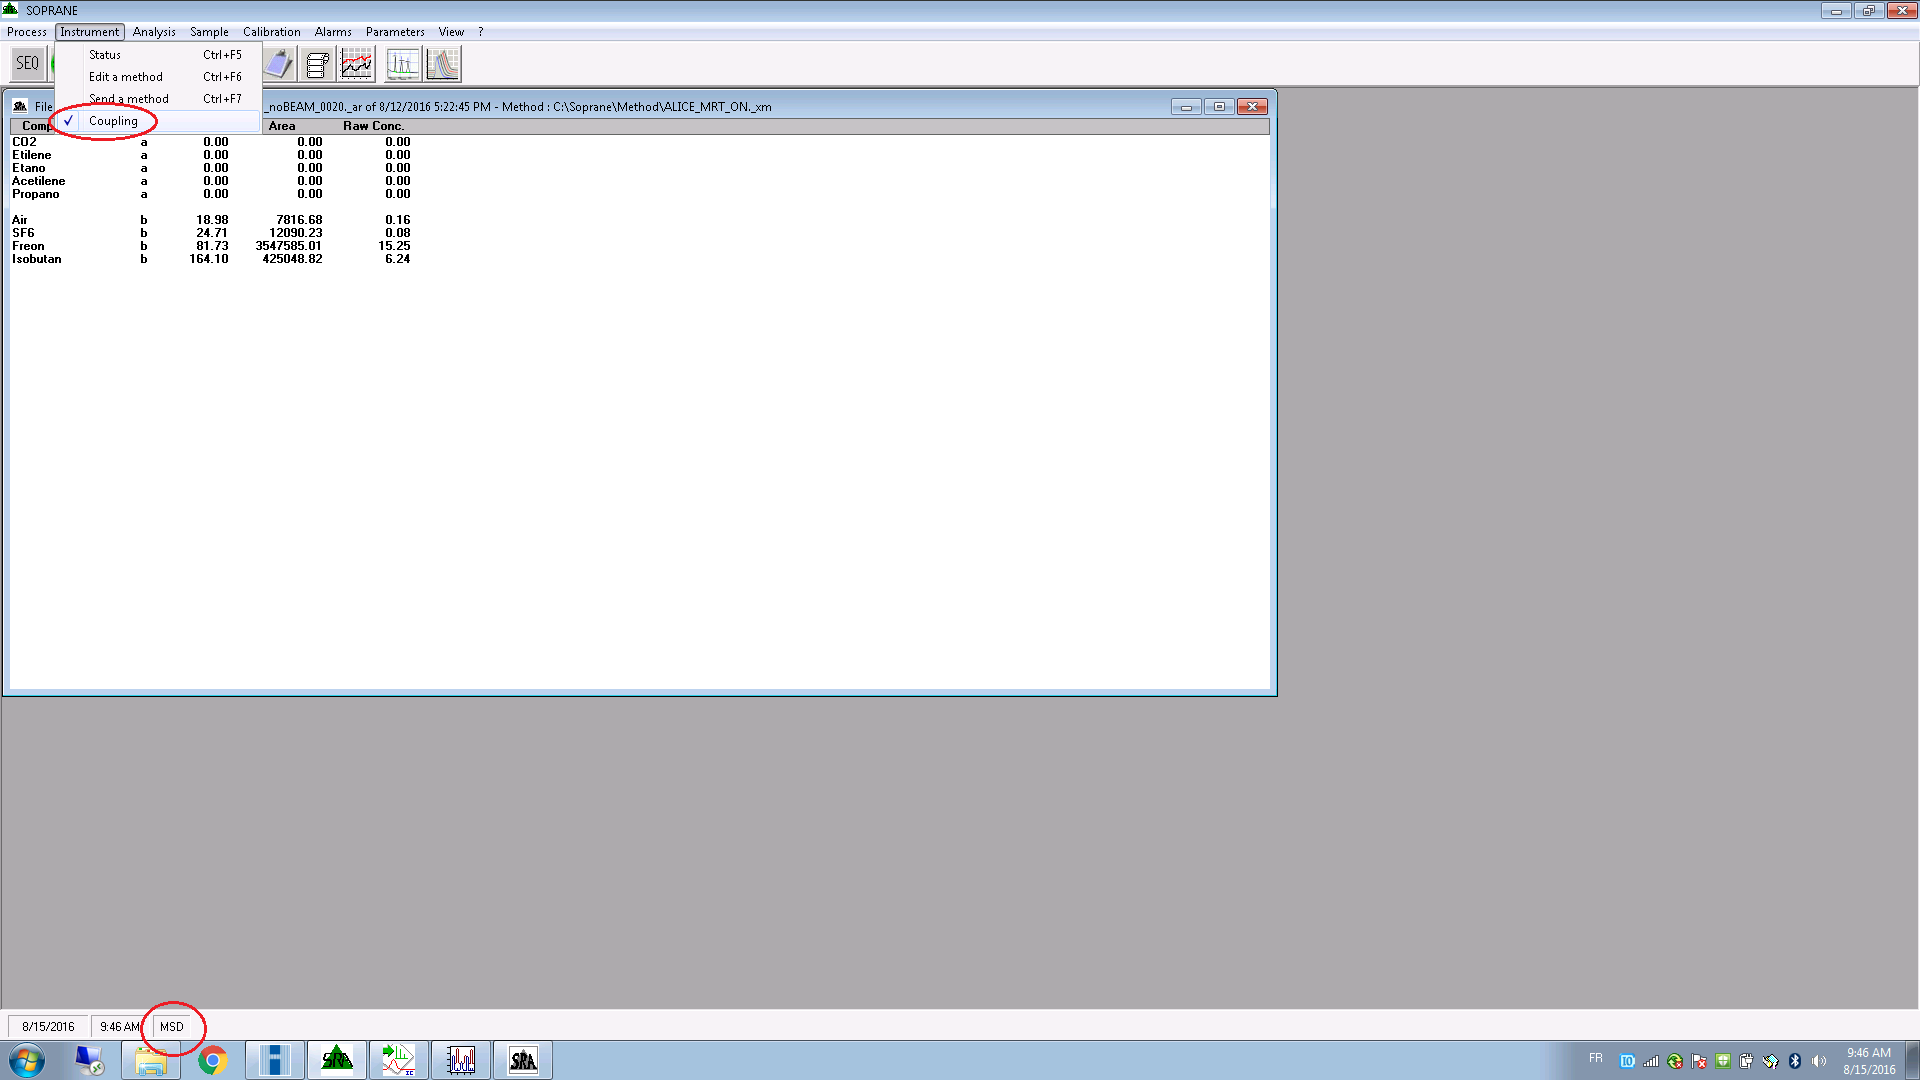
\includegraphics[width=1.2\textwidth]{4CheckSoprane.png}
\label{fig:univerise}
\end{figure}

Then start an analysis and wait for the MSD to go into PreRun mode, a window should pop-up that would allow you to manually start the MS analysis; don't press it. Now the MSD is in the required state and we can continue configuring the trigger properly.

\newpage

 Close Soprane software, then open Soprane setup software and go \texttt{Test -> Remote Relay}. If this option bring an error, please configure the Pumps correctly, to do that you should follow the procedure described in section: \texttt{Solving common problems: Configuring the pumps correctly} at the end of this guide.

\begin{figure}[h]
\centering
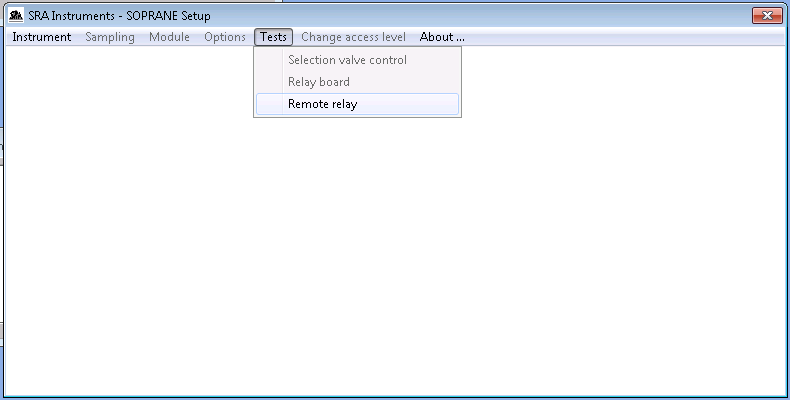
\includegraphics[width=1\textwidth]{5SopraneSetupTest.png}
\label{fig:univerise}
\end{figure}

After clicking there you should be greeted with a new window similar to the one shown just below this lines. This window allows the user to manually trigger the relays corresponding to the cable connecting the GC and the MSD. It will allow us to test which of the outputs (relays) in connected to the "Start analysis trigger" so that we will be able later to tell the GC which one to activate when a GC+MSD analysis is to be performed.

\begin{figure}[h]
\centering
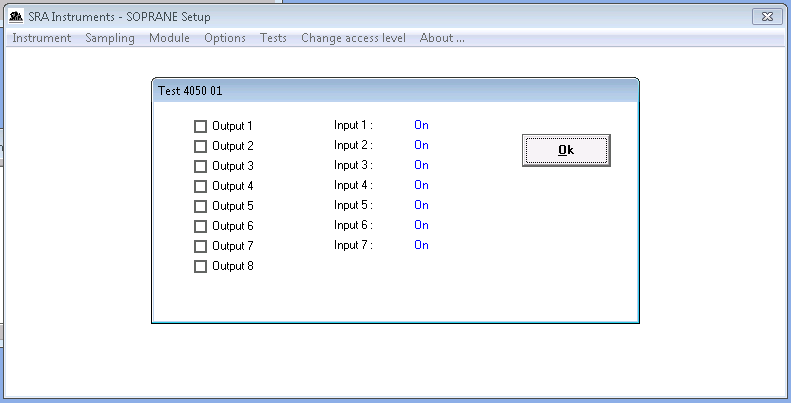
\includegraphics[width=1\textwidth]{6RelayBoard.png}
\label{fig:univerise}
\end{figure}



\section{Finding out the relay that triggers the analysis}

Now it's time to find out which relay triggers the analysis. For that we will have to keep an eyes on the MSD Chemstation while we start ticking the boxes on the relay board in Soprane Setup. After we tick a box we should wait about 2-3seconds to see if it had any impact on the MSD Chemstation. Remember that the MSD Chemstation should be in "\texttt{PreRun} Mode" for the triggers to possible have any effect.

\begin{figure}[h]
\centering
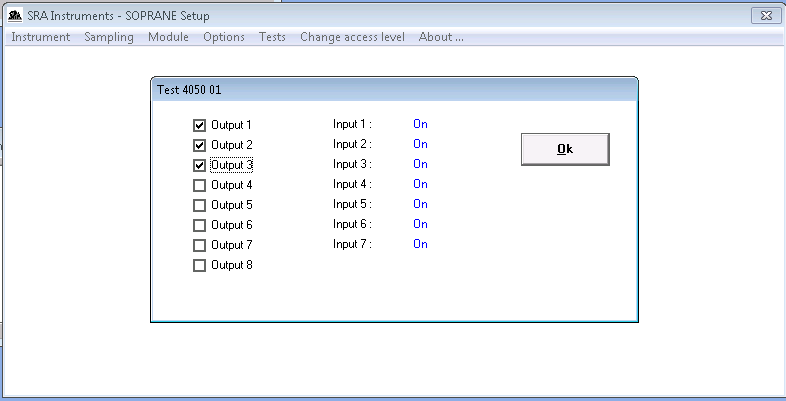
\includegraphics[width=.7\textwidth]{7TickingRelays.png}
\label{fig:univerise}
\end{figure}

When you find the trigger relay you should see something similar to the picture underneath this lines where after we checked \texttt{Output 4} the MSD went from \texttt{PreRun} to \texttt{Run} state, meaning the analysis was started by this 4th output, i.e. the 4th relay is the one that triggers the analysis. Keep that number in mind since that's what we will need to configure the automatic synchronisation of the GC and the MSD.

\begin{figure}[h]
\centering
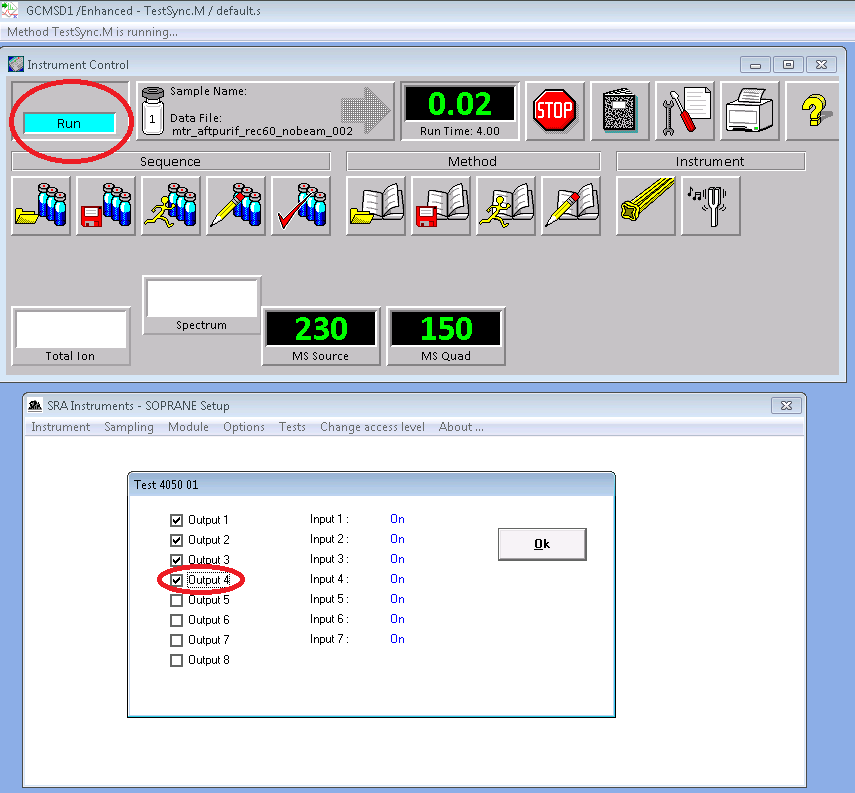
\includegraphics[width=.6\textwidth]{8FindTrigger.png}
\label{fig:univerise}
\end{figure}
\newpage

\section{Configuring the syncing process}

After one has found the trigger for analysis it's time to configure it so that Soprane will trigger said relay at the beginning of the GC analysis making the MSD start in sync with it. We shall untick all the check-boxes and hit \texttt{OK}.

One should now go back to Soprane Setup starting screen and select \texttt{Options -> Analysis} as shown below.

\begin{figure}[h]
\centering
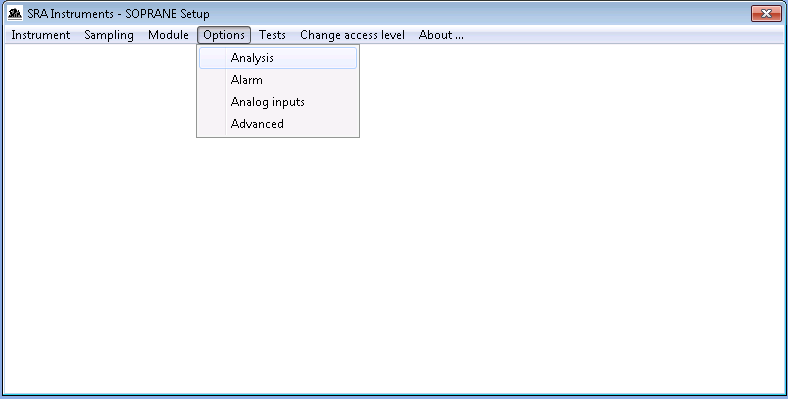
\includegraphics[width=.9\textwidth]{9SetupAnalysis.png}
\label{fig:univerise}
\end{figure}


Then a new window will pop-up. We aim to configure the options under \texttt{Management of the external start output} with the right values.

\begin{figure}[h]
\centering
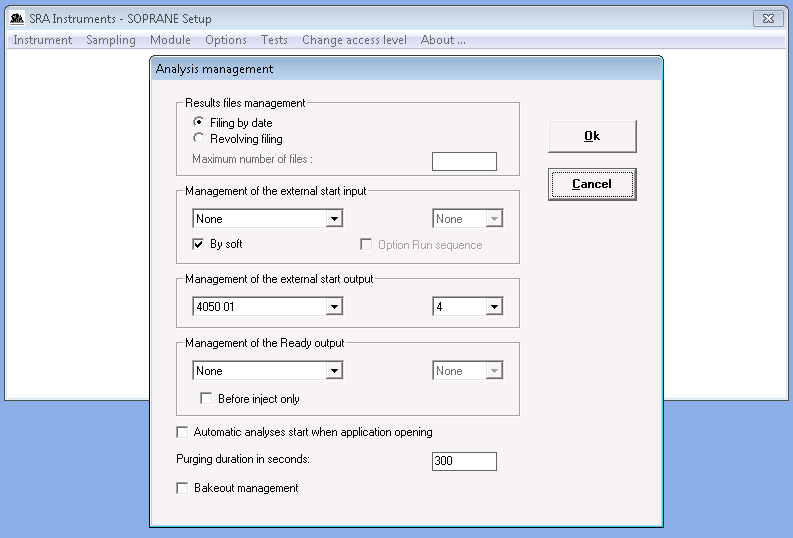
\includegraphics[width=.9\textwidth]{10ConfigureTrigger.png}
\label{fig:univerise}
\end{figure}

\newpage

The first box should be filled with the ID of the relay board which is what appeared as window title when we searched for the trigerring relay. The number on the right corresponds to the actual relay and it's the one that triggers the analysis, so following the previous example it would be number 4.

\begin{figure}[h]
\centering
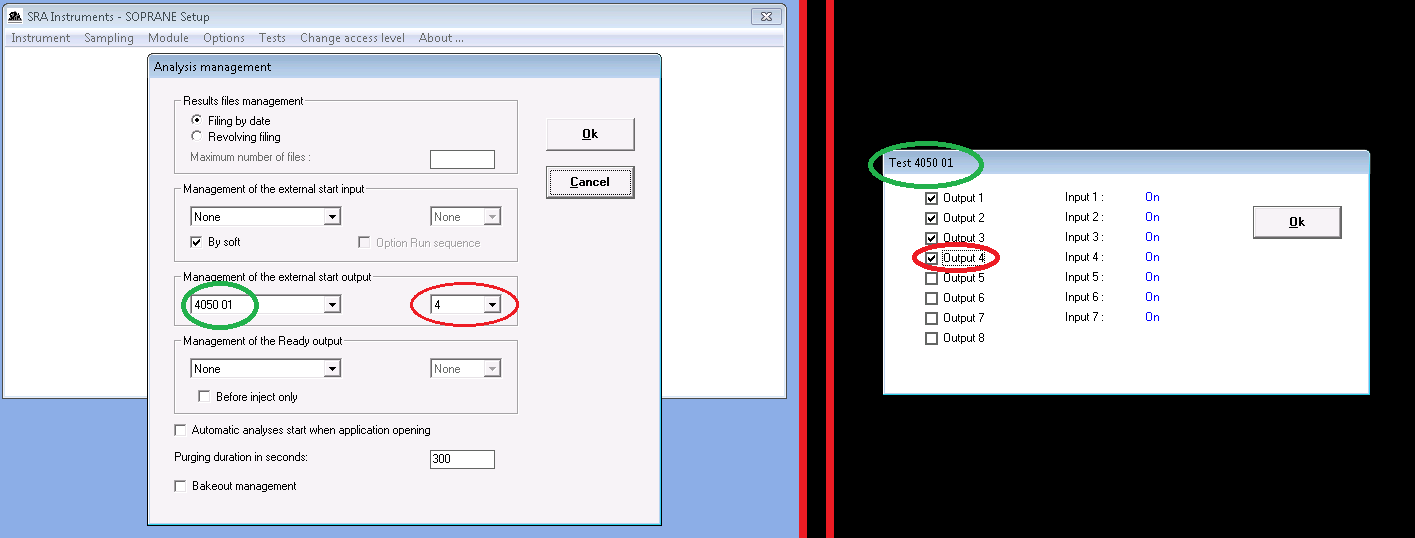
\includegraphics[width=1.2\textwidth]{11CorrectOptions.png}
\label{fig:univerise}
\end{figure}


We now hit \texttt{OK} and close Soprane Setup saving changes. The configuration process is done. It is recommended to perform a test analysis to check that everything went correctly.

Also one could/should revert the changes in the MSD triggering and change from \texttt{Manual} to \texttt{External Device}. This will change nothing in the analysis process but will prevent the MSD from creating additional windows for triggering a manual start of the MSD analysis.

\newpage

\section{Solving common problems: Configuring the pumps correctly}

It might happen that the pumps and relay board are not configured correctly, even if the pump is working for the analysis. This will be apparent when trying to access the test window of the relay board as you will get an error message and will not be able to see said relay testing window.

Once we have check that the pump needs some configuration we click on \texttt{Module -> Remote modules -> Adam and + ..} 

\begin{figure}[h]
\centering
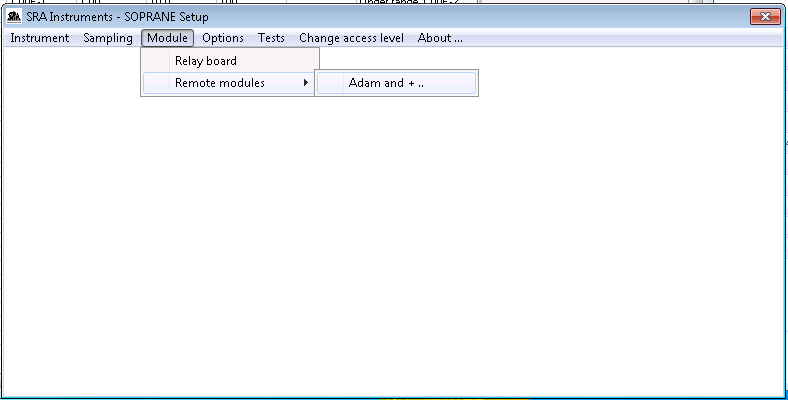
\includegraphics[width=.9\textwidth]{12AddRemote.png}
\label{fig:univerise}
\end{figure}

A configuration window for the attached devices will appear before us and we should now proceed to configure correctly our pump. At this point it's important to know how many pumps we have so that we can cross check if everything is properly configured.

\begin{figure}[h]
\centering
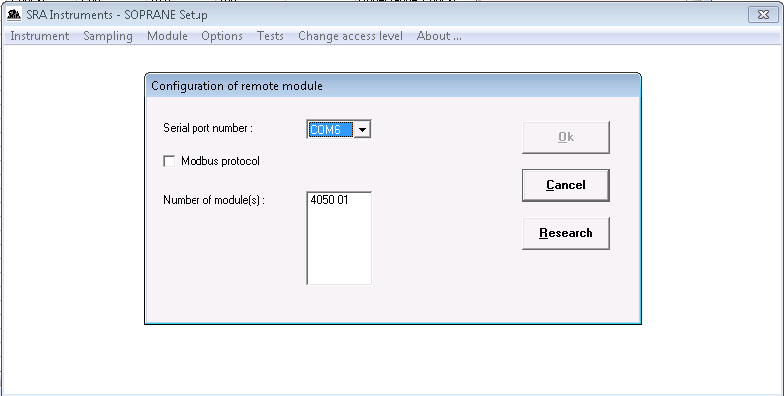
\includegraphics[width=.9\textwidth]{13ComConfig.png}
\label{fig:univerise}
\end{figure}

When presented with the screen we can start finding the right COM port where the pump and relay board are connected. For that we try each of the different
\end{document}
